\documentclass[12pt, a4paper]{article}

% -----------------------------
% PACKAGES
% -----------------------------
\usepackage{graphicx}
\usepackage[utf8]{inputenc}
\usepackage[T1]{fontenc}
\usepackage{lmodern}
\usepackage[left=2.5cm, right=2.5cm, top=3cm, bottom=3cm]{geometry}
\usepackage{booktabs}
\usepackage{array}
\usepackage{tabularx}
\usepackage{amsmath}
\usepackage{hyperref}
\usepackage{enumitem}
\usepackage{float}
\usepackage{caption}
\usepackage{setspace}
\usepackage{parskip}
\usepackage{fancyhdr}
\usepackage{titlesec}
\usepackage{color}
\usepackage[table]{xcolor}
\usepackage{listings}
\usepackage{url}
\usepackage{multirow}
\usepackage{colortbl}

% -----------------------------
% COLORS
% -----------------------------

\definecolor{solarblue}{RGB}{31, 78, 121}
\definecolor{solaramber}{RGB}{180, 100, 20}
\definecolor{solargray}{RGB}{80, 80, 80}
\definecolor{lightgray}{RGB}{245, 245, 245}
\definecolor{codebg}{RGB}{248, 248, 248}

% -----------------------------
% SECTION STYLE
% -----------------------------

\titleformat{\section}{\large\bfseries\color{solarblue}}{}{0em}{\thesection\quad}[\titlerule]
\titleformat{\subsection}{\normalsize\bfseries\color{solaramber}}{}{0em}{\thesubsection\quad}
\titleformat{\subsubsection}{\normalsize\itshape\color{solargray}}{}{0em}{\thesubsubsection\quad}

% -----------------------------
% HYPERREF
% -----------------------------

\hypersetup{
    colorlinks=true,
    linkcolor=solarblue,
    urlcolor=solaramber,
    citecolor=solarblue
}

% -----------------------------
% HEADER / FOOTER
% -----------------------------

\pagestyle{fancy}
\fancyhf{}
\fancyhead[R]{\small\textit{Vehicle Maintenance Prediction \& Agentic Fleet}}
\fancyfoot[C]{\thepage}
\renewcommand{\headrulewidth}{0.4pt}

% -----------------------------
% SPACING
% -----------------------------

\onehalfspacing
\setlength{\parindent}{0pt}

\begin{document}

% ---------------------- TITLE PAGE ----------------------
\begin{titlepage}
    \centering
    \vspace*{2cm}

    {\Large \textbf{PROJECT 6}}\\[1.2cm]

    {\Huge\bfseries\color{solarblue}
    Vehicle Maintenance Prediction}\\[0.5cm]

    {\Large\bfseries\color{solaramber}
    \& Agentic Fleet Management}\\[0.8cm]

    \rule{\linewidth}{1.2pt}\\[0.8cm]

    {\large From Predictive Maintenance to Autonomous Fleet Operations}

    \vspace{1.5cm}

    \begin{tabular}{l}
        \textbf{Team Members:} \\
        Milind Bansal \\
        Isha Tomar \\
        Yashi Agrawal \\
        Mansi Agarwal \\
    \end{tabular}

    \vspace{1cm}

    \textbf{Section:} D \\[0.2cm]
    \textbf{Faculty:} Kartik Gupta

    \vfill
    \today
\end{titlepage}
\newpage

% ---------------------- ABSTRACT ----------------------

\begin{abstract}
\noindent
Modern fleet operations generate continuous streams of operational telemetry data including mileage, engine load, vibration, temperature, and environmental conditions. However, maintenance decisions are frequently based on fixed schedules or reactive breakdown-based strategies. These approaches fail to incorporate real-time operational stress and vehicle-specific conditions.

This project presents an end-to-end supervised machine learning framework for predicting whether a vehicle requires maintenance. Unlike traditional binary classification problems, this task represents a risk-detection scenario where false negatives may result in breakdowns, downtime, financial loss, and safety hazards. Therefore, evaluation prioritizes recall, F1-score, and ROC-AUC over simple accuracy.

The dataset consists of 15,000 structured vehicle records with 28 engineered and encoded features. Extensive exploratory data analysis, correlation study, outlier handling, and feature engineering were conducted before model training. Four classification models were implemented and compared: Logistic Regression, Decision Tree, Random Forest, and XGBoost.

After hyperparameter optimization using RandomizedSearchCV, the tuned XGBoost classifier achieved an ROC-AUC of 0.92 and balanced minority-class recall performance. 

To transition from predictive analytics to prescriptive operational intelligence, the deployment architecture securely incorporates an autonomous Agentic Fleet Management system. Using LangGraph, this agent integrates the machine learning predictions with Retrieval-Augmented Generation (RAG), rule-based diagnostics, and a Large Language Model (LLM) to generate actionable and contextual maintenance plans via an interactive Streamlit framework.

Ultimately, this work demonstrates a complete, production-grade intelligence pipeline bridging the gap between data preprocessing and autonomous decision execution.
\end{abstract}
\newpage

% ---------------------- CONTENTS ----------------------

\tableofcontents
\newpage

\section{Introduction}

Fleet maintenance is traditionally performed either at fixed service intervals or after mechanical failure occurs. Fixed scheduling ignores real operational stress, while reactive maintenance increases downtime and operational risk.

The core predictive problem addressed in this project is:

\textit{Can historical vehicle telemetry data be used to proactively predict whether a vehicle requires maintenance?}

This is not merely a classification problem; it is a risk-sensitive detection problem. A false negative — failing to detect required maintenance — may result in:

\begin{itemize}
\item Unexpected mechanical breakdown
\item Operational downtime
\item Increased repair costs
\item Safety hazards
\end{itemize}

Beyond prediction, this project formally addresses the prescriptive challenge: \textit{what action should be taken when a risk is detected?} By embedding the predictive ML model into a stateful, LLM-powered agent workflow, the system moves beyond merely predicting failure. It actively and autonomously diagnoses subsystems, interprets recurring variables, and outputs precise maintenance procedures.

\section{Dataset Description}

The dataset consists of structured vehicle telemetry features collected from simulated fleet operations.

\begin{table}[H]
\centering
\caption{Dataset Overview}
\begin{tabular}{ll}
\toprule
Property & Value \\
\midrule
Total Samples & 15,000 \\
Target Variable & Maintenance Required (0/1) \\
Class Distribution & 75\% No Maintenance, 25\% Maintenance \\
Raw Numerical Features & 10 \\
Categorical Features & 5 \\
Total Features After Encoding & 28 \\
\bottomrule
\end{tabular}
\end{table}

\section{Exploratory Data Analysis}

\subsection{Feature Scale Variation}

The statistical summary revealed significant variation in feature magnitudes. For example:
\begin{itemize}
\item Mileage ranged in tens of thousands.
\item Battery voltage ranged within a narrow band.
\item Vibration levels were tightly distributed.
\end{itemize}
This influenced the need for scaling in linear models during preprocessing.

\subsection{Outlier Detection}

Boxplot analysis revealed extreme upper tails in mileage and engine hours. Instead of removing these records, IQR-based capping was applied because high-usage vehicles represent realistic operational scenarios.

\subsection{Class Imbalance}

The dataset exhibited moderate imbalance (~75:25). Accuracy alone would therefore be misleading. For example, predicting all vehicles as "No Maintenance" yields 75\% accuracy without predictive power. Thus, Recall and F1-score were heavily prioritized throughout the model evaluation.

\begin{figure}[H]
    \centering
    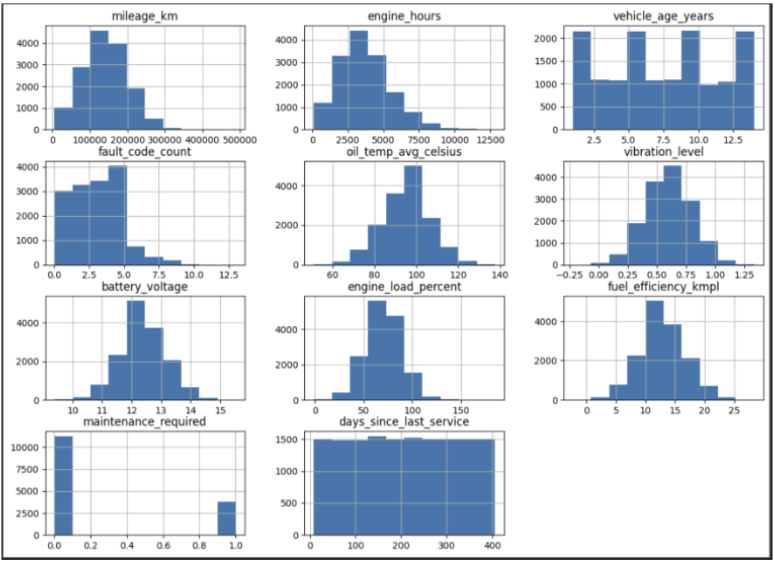
\includegraphics[width=0.6\linewidth]{images/ValueRange.png}
    \caption{Distribution and Values Range for Telemetry Variables}
    \label{fig:Values Range}
\end{figure}

\begin{figure}[H]
    \centering
    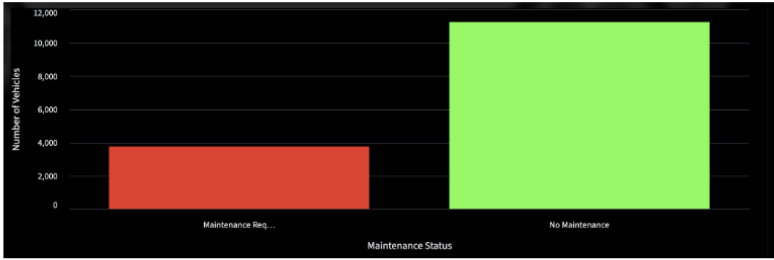
\includegraphics[width=0.6\linewidth]{images/ClassImbalance.png}
    \caption{Class Imbalance in Target Variable}
    \label{fig:Class Imbalance}
\end{figure}

\begin{figure}[H]
    \centering
    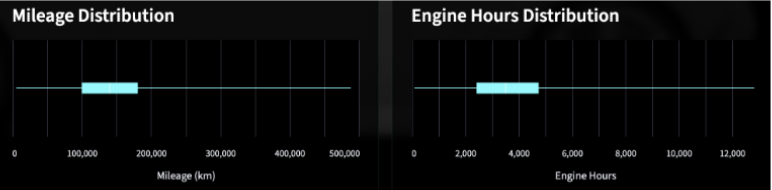
\includegraphics[width=0.6\linewidth]{images/BoxPlot.png}
    \caption{Box Plot indicating underlying distributions and bounds}
    \label{fig:Box Plot}
\end{figure}

\newpage
\section{Feature Engineering}

Raw telemetry features often fail to capture the interaction effects and operational intensity patterns that influence mechanical degradation. Therefore, domain-informed feature engineering was performed within the \texttt{utils/preprocessor.py} logic to transform primary signals into more meaningful stress indicators.

\subsection{Rationale for Feature Engineering}

Vehicle maintenance requirements are rarely triggered by a single variable in isolation. Instead, risk emerges from compounded operational stress, long-term wear, and contextual environments. 
For example:
\begin{itemize}
\item High mileage accumulated slowly over 10 years does not represent the same stress as high mileage accumulated within 2 years.
\item High engine load under normal temperature may be acceptable, but high load combined with elevated temperature significantly accelerates thermal wear.
\end{itemize}

\subsection{Engineered Features}

\begin{table}[H]
\centering
\caption{Engineered Feature Summary}
\begin{tabularx}{\textwidth}{lX}
\toprule
\textbf{Feature} & \textbf{Rationale and Interpretation} \\
\midrule
\texttt{mileage\_per\_year} & Measures operational intensity rather than absolute mileage. Captures aggressive usage relative to vehicle age. \\
\texttt{engine\_hours\_per\_km} & Indicates workload per distance traveled. High values reflect inefficient combustion or idle-heavy operations. \\
\texttt{fault\_density} & Normalizes fault frequency relative to engine hours, capturing returning mechanical instability. \\
\texttt{thermal\_stress} & Computed as oil temperature $\times$ engine load. Highlights compounded strain under operational loads. \\
\texttt{load\_efficiency} & Ratio of engine load to fuel efficiency. Identifies elevated mechanical strain mapping dynamically to performance outputs. \\
\bottomrule
\end{tabularx}
\end{table}

\subsection{Validation Through Feature Importance}

After training tree-based models, parameter importance analysis confirmed that \texttt{thermal\_stress}, \texttt{fault\_code\_count}, and \texttt{mileage\_per\_year} ranked among the most predictive variables, validating the engineering logic empirically.

\newpage
\section{Model Training and Selection Strategy}

To evaluate model complexity reliably, a progressive approach established benchmarks across linear, rules-based, and ensemble frameworks. 

\subsection{Train-Test Split}

The dataset was divided using an 80/20 train-test split via stratified sampling, preserving the minority maintenance class distributions perfectly within both cross-validation stages.

\subsection{Progressive Model Evaluation}

\textbf{Logistic Regression (Baseline):} Served as an interpretable linear benchmark. Though it achieved high baseline accuracy, its recall for the maintenance class remained low, proving the data's underlying bounds were highly non-linear.

\textbf{Decision Tree:} Brought non-linear segmentation to the pipeline. While providing clear logical conditions, it notably suffered from high variance and reduced ROC-AUC, confirming overfitting.

\textbf{Random Forest:} Radically stabilized variances by bagging trees trained on sub-sampled data branches. It restored ROC-AUC levels impressively but still struggled with aggressive minority class identification.

\textbf{XGBoost (Final Selected Model):} Leveraging a rigorous gradient boosting strategy, this classifier corrected residual classification errors iteratively. Using integrated \texttt{scale\_pos\_weight} parameters, the framework naturally amplified loss gradients against false negatives, successfully capturing imbalanced targets with high stability.

\subsection{Hyperparameter Optimization Strategy}

Hyperparameters were strictly formulated via random searching (\texttt{RandomizedSearchCV}), focusing on balancing the precision-recall trade-off through 3-fold cross validation. 
Optimized constraints included:
\begin{itemize}
    \item \texttt{n\_estimators} and \texttt{max\_depth}
    \item \texttt{subsample} and \texttt{learning\_rate}
    \item \texttt{scale\_pos\_weight} (critical for combating the 75:25 dataset imbalance).
\end{itemize}

\subsection{Model Comparison Summary}

\begin{table}[H]
\centering
\caption{Model Performance Comparison on Test Set}
\begin{tabular}{lcccc}
\toprule
Model & Accuracy & Recall & F1-Score & ROC-AUC \\
\midrule
Logistic Regression & 0.84 & 0.60 & 0.68 & 0.92 \\
Decision Tree & 0.83 & 0.60 & 0.66 & 0.85 \\
Random Forest & 0.85 & 0.58 & 0.70 & 0.91 \\
\rowcolor{solarblue!8}
\textbf{XGBoost (Tuned)} & \textbf{0.85} & \textbf{0.76} & \textbf{0.78} & \textbf{0.92} \\
\bottomrule
\end{tabular}
\end{table}

By successfully capturing a recall rate of 0.76 and ROC-AUC of 0.92, XGBoost was selected for system deployment.

\newpage
\section{Agentic Fleet Management Architecture}

Transitioning from isolated predictive metrics to intelligent, prescriptive automation required embedding the serialized ML model within a sophisticated cognitive workflow. Located fundamentally within the \texttt{utils/} package architecture, the Agentic Fleet Management system orchestrates raw predictions alongside empirical diagnostic heuristics, context-aware semantic retrieval, and local generative processing.

\subsection{Agent Components and State Graph Integration}

The decision environment executes as a stateful, directed acyclic \texttt{StateGraph} managed securely via the LangGraph framework (\texttt{utils/langgraph\_agent.py}). The agent injects predictive queries through a sequence of discrete operational nodes:

\begin{enumerate}
    \item \textbf{Validation Node (\texttt{validate}):} Serves as the primary defensive barrier for the application. It parses explicit text variables—such as "abnormal vibrations" or "hot engine"—from operator maintenance prompts and forces corresponding values programmatically over the base telemetry dataset. From here, the integrated data passes to \texttt{validate\_vehicle\_input()} to guarantee all standardizations apply faithfully before scoring.
    
    \item \textbf{Scoring Node (\texttt{score}):} Re-instantiates and executes the core XGBoost estimator algorithm (\texttt{utils/model\_tool.py}). Upon calculating the raw algorithmic risk vectors, this node executes a rigid extraction loop testing the values across hard-coded subsystem thresholds. Output metrics directly derive tangible semantic signals, effectively mapping "risk\_110\_temp" directly into actionable definitions of "Thermal Stress" and subsequent component vulnerabilities.
    
    \item \textbf{Retrieval Node (\texttt{retrieve}):} The engine uses Retrieval-Augmented Generation (RAG). Supported context paths within \texttt{utils/retriever.py} launch a localized semantic query searching the designated vector space. Relevant domain protocols matching the detected fault signals merge to define exact manuals and best-practice timelines needed by the vehicle operator.
    
    \item \textbf{Reporting Node (\texttt{report}):} Operates as the synthesis endpoint (\texttt{utils/agent\_logic.py}). Combining the quantitative risks and generated queries, the agent creates a programmatic \texttt{action\_plan}. It formalizes timeline advice, assesses fleet policy compliance (SLA service requirements, lifecycle triggers), and structures the service outlook securely.
\end{enumerate}

\subsection{LLM Orchestration and Generative Enrichment}

Crucially, the finalized report matrices process through a dynamic enrichment loop (\texttt{maybe\_enrich\_with\_llm}). Bridging external intelligence via local \texttt{ChatOllama} frameworks, the system refines structured technical payloads into consumable linguistic directives and conversational diagnostic responses.

By relying on LangGraph and empirical guardrails throughout the inference flow, risk probabilities generated by XGBoost bind tightly against factual system schemas, preventing standard generative hallucination gaps common in unmodified LLMs.

\newpage
\section{End-to-End System Workflow}

The pipeline executes holistically, establishing an immediate feedback loop bridging physical vehicle telemetry with cognitive, automated dispatch intelligence. System integrity relies heavily on a tightly coupled software architecture.

\subsection{Actual Execution Flow}

\begin{enumerate}
    \item \textbf{Streamlit Input:} Telemetry and free-form queries aggregate within localized frontend interfaces (\texttt{Home.py} / \texttt{pages/} / \texttt{app.py}).
    \item \textbf{Feature Engineering and Preprocessing:} The \texttt{utils/preprocessor.py} matrix aligns schemas properly to internal vectors, enforcing encoding limits.
    \item \textbf{Machine Learning Layer:} State nodes query the serialized \texttt{models/vehicle\_model.joblib}.
    \item \textbf{Graph Orchestration (LangGraph):} XGBoost probabilities route into \texttt{utils/langgraph\_agent.py}, triggering logic and rule-based diagnostic signals.
    \item \textbf{Vector Retrieval (RAG):} \texttt{utils/retriever.py} filters relevant structural knowledge bases dynamically referencing the identified vulnerabilities.
    \item \textbf{Generative Agent Delivery:} The reporting nodes bundle, format, LLM-enrich, and render comprehensive prescriptive fleet instructions seamlessly back to the UI.
\end{enumerate}

\begin{figure}[H]
    \centering
    % \includegraphics[width=0.95\textwidth]{images/diagram.png}
    \rule{0.95\textwidth}{8cm} % Placeholder for diagram.png
    \caption{Complete end-to-end Machine Learning \& Agentic Diagnostic Flow architecture}
    \label{fig:architecture_diagram}
\end{figure}

\newpage
\section{Repository Architecture}

To ensure sustainable production scaling, the repository segregates functional components deliberately:

\begin{table}[H]
\centering
\caption{Project Directory and Component Layout}
\begin{tabularx}{\textwidth}{lX}
\toprule
\textbf{Path / Location} & \textbf{Primary Purpose and Alignment} \\
\midrule
\textbf{\texttt{data/}} & Contains processed training telemetry structures needed for standardizations.\\
\textbf{\texttt{models/}} & Secures the exact, serialized predictive machine learning artifacts (\texttt{.joblib}). \\
\textbf{\texttt{utils/}} & The core analytical backbone—houses \texttt{agent\_logic.py}, \texttt{langgraph\_agent.py}, \texttt{retriever.py}, \texttt{config.py}, bridging the gap between web UI and underlying cognitive modeling strings.\\
\textbf{\texttt{app.py} / \texttt{Home.py}} & Streamlit frontend execution protocols handling system-client network layers.\\
\textbf{\texttt{report/}} & Formal documentation frameworks ensuring technical transparency. \\
\textbf{\texttt{walkthrough/}} & Base research files representing experimental exploratory tests initially forming model baseline arguments. \\
\textbf{\texttt{assets/}} & Graphic styling utilities bridging interactive CSS variables required by the system interface.\\
\bottomrule
\end{tabularx}
\end{table}

\section{Technology Stack}

\begin{table}[H]
\centering
\caption{Technology Stack Overview}
\begin{tabular}{ll}
\toprule
\textbf{Layer} & \textbf{Technology} \\
\midrule
Data Preprocessing \& Pipeline & pandas, NumPy, scikit-learn \\
Model Generation Frameworks & XGBoost, RandomizedSearchCV \\
Agentic System Workflow & LangGraph, Langchain \\
Generative Intelligence \& Retrieval & ChatOllama, Chroma Vector Search \\
Deployment \& Web Interface & Streamlit, HTML/CSS Integrations \\
System Persistence & joblib \\
\bottomrule
\end{tabular}
\end{table}

\section{Conclusion}

\begin{center}
\colorbox{solarblue!8}{\parbox{0.9\textwidth}{\centering
\textbf{\color{solarblue}Operational Achievement:} By coupling a robust XGBoost risk-estimator capable of 0.92 ROC-AUC predictability directly into a deterministic LangGraph agentic chain, this solution radically upgrades asset management platforms constraints from passive binary identification systems to fully capable, prescriptive, and cognitive autonomous operational fleet dispatchers.
}}
\end{center}

This implementation firmly bridges the data science capabilities of precision telemetry encoding directly against actionable, stateful, and context-aware generative artificial intelligence.

\section{References}
\begin{thebibliography}{9}

\bibitem{github}
Vehicle Maintenance Predictor \& Agentic Platform – GitHub.  
\url{https://github.com/11yashiagrawal/vehicle_maintenance_dashboard}

\bibitem{langgraph}
LangGraph framework references for Stateful Execution mapping.
\url{https://python.langchain.com/docs/langgraph}

\bibitem{liveapp}
Vehicle Maintenance Predictor – Live Deployment Target.  
\url{https://vehicle-maintenance-dashboard.streamlit.app/}

\end{thebibliography}
\end{document}
